\section{Introduction}
\label{sec:intro}

Agents that operate scientific experiments must do more than answer questions about a
finished table. They choose what to run, allocate scarce physical capacity, interpret
partial and noisy evidence, and decide when that evidence supports an operating
recommendation. Existing work evaluates important parts of this loop: BoxingGym limits
sequential experimentation and measures information gain, Olympus and Summit expose
executable optimisation surfaces, Minerva studies noisy parallel batches, and budgeted or
delayed-feedback Bayesian optimisation formalises cost and latency
\citep{boxinggym,olympus,summit,minerva,astudillo2021budgeted,verma2022delayed}. The combined
decision remains difficult to measure when trials occupy a tiered facility, poor experiments
lose real objective value, and a submitted treatment cannot be recalled.

\slowlab{} makes that decision executable in controlled-environment horticulture. A site is
drawn from a documented crop-and-economics distribution. An agent assigns treatments to
named chambers and hydroponic loops, commits them for a 210-day crop cycle, observes only
measurements available by the current simulation time, and recommends an operating point.
Chamber-level climate controls and loop-level cultural controls create a split-plot action
space: replication, treatment coverage, and physical placement compete for the same units.
The published TOMGRO crop model supplies traceability rather than author-independent
difficulty; budgets, ranges, observation channels, and site distributions remain explicit
benchmark choices \citep{jones1999reduced}.

We organise the benchmark around three roles (Figure~\ref{fig:roles}). A \emph{design
policy} chooses treatments and their physical allocation. A \emph{history reader} maps the
time-stamped visible record to a recommendation. A closed-loop agent may implement both in
one model, but fixed-history replay can vary one role while holding the other fixed. The
\emph{evaluator} belongs to the benchmark, may use hidden truth to score the submitted
outputs, and never returns privileged information to the agent.

\begin{figure}[t]
\centering
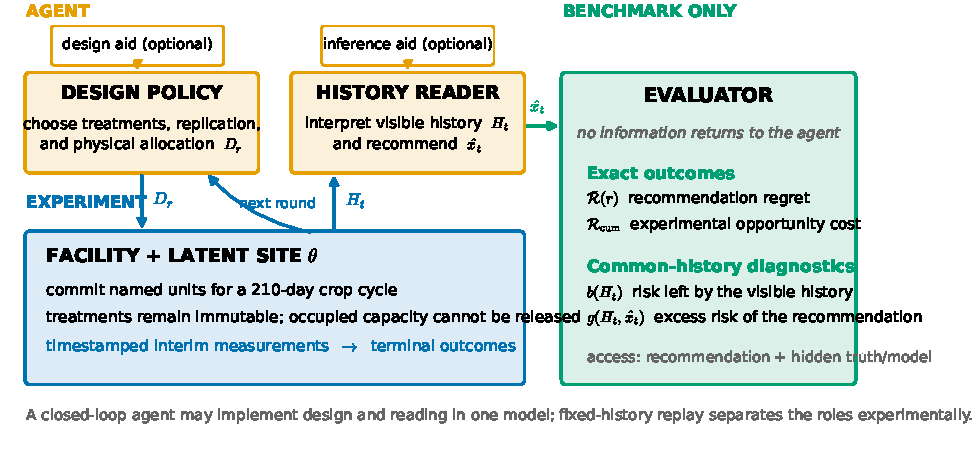
\includegraphics[width=\linewidth]{figures/roles_information_flow.pdf}
\caption{\textbf{Roles and information flow.} The design policy commits treatments and
physical units; the history reader sees only the time-stamped history and produces a
recommendation. The benchmark-side evaluator computes exact outcomes from hidden truth and
calibrated diagnostics from the same visible history. Interim observations may update the
reader and the next design, but cannot alter a committed treatment or release capacity.}
\label{fig:roles}
\end{figure}

Our contribution is threefold. First, we formulate scientific-agent evaluation as coupled
allocation, evidence-use, and recommendation problems under slow, noisy, costly, and
irreversible feedback. Second, we define an information boundary and a common-history
diagnostic that separates what the executed design could support from how the reader used
that evidence. Third, we test scripted policies and model agents in frozen, site-paired
experiments. The resulting claim is deliberately bounded: the tested aids show no reliable
improvement in the primary setting, one lower-noise condition shows harm, and the relative
importance of allocation and reading varies by task.
